% !TeX root = ../translation.tex

\section{GAN和最优传输}

OT理论为GANgan奠定了理论基础。许多最近的工作,如WGAN[1],WGAN-GP[27],和RW-GAN[47],使用瓦瑟斯坦距离来测量生成的数据分布和真实数据分布之间的偏差。

从OT的角度来看,生成器和鉴别器的最优解以一种封闭的形式联系起来;因此,生成器和鉴别器应该协作而不是竞争。更多细节请参见参考文献。[11].此外,Monge-Ampère解的正则性理论可以解释GAN[48]中的模态坍缩。

\subsection{竞争与合作}

WGAN[1]的OT视图如图 \ref{fig:2} 所示。根据流形分布假设,真实数据分布$\nu$接近于嵌入在环境空间$\chi $中的流形$\sum$。生成器计算从潜在空间$Z$到环境空间的解码映射$g_\theta$,并将白噪声$\zeta$(即高斯分布)转换为生成的分布$\mu _{\theta}$。该鉴别器通过计算坎托罗维奇的潜在$\varphi _{\zeta}$,计算$\mu _{\theta}$与真实数据分布$\nu$,$W_c(\mu _{\theta},\nu)$之间的瓦瑟斯坦距离。$g_{\theta}$和$\varphi _{\zeta}$都是由DNN实现的。

在训练过程中,生成器改善$g_{\theta}$通过$(g_{\theta})_{\#} \zeta$来更好地近似$\nu$;鉴别器改进了坎托洛维奇势$\varphi _{\zeta}$以改进对瓦瑟斯坦距离的估计。生成器和鉴别器相互竞争,而不共享中间的计算结果。在$L^1$成本函数下,WGAN的替代训练过程可以表述为期望的最小-最大优化:
\begin{equation*}
	\min_{\theta } \max_{\xi } E_{z\sim \zeta } \left \{ \varphi _{\xi } \left [ g_{\theta } (z) \right ]   \right \} + E_{y\sim \nu}\left [ \varphi_{\xi}^c (y) \right ]  
\end{equation*}

但如果我们将代价函数改变为$L^2$距离,那么根据定理(\ref{theorem:3.2}),在最优时,布雷尼尔的势$\mu$和康塔洛维奇的势$\varphi$通过等式(\ref{function:16})的封闭形式 $u(x)=\frac{1}{2} \left \| x \right \|^2 -\varphi(x)$ 联系起来, 生成器追求OT映射$\bigtriangledown u$;鉴别器计算$\varphi$。因此,一旦生成器达到最优值,无需任何训练就可以得到鉴别器的最优解,反之亦然。

更详细地说,假设在第$k$次迭代时,生成器映射为$g_{\theta}^k$。鉴别器计算康塔洛维奇势$\varphi_{\zeta}$,给出当前生成的数据分布$\left ( g_{\theta}^k \right )_{\#} \zeta $和真实数据分布$\nu$之间的瓦瑟斯坦距离;$\bigtriangledown u$给出从$\left ( g_{\theta}^k \right )_{\#} \zeta $到 $\nu$的OT映射。因此,我们得到了以下结果:
\begin{equation*}
	v=(\bigtriangledown u)_{\#} \left [ \left ( g_{\theta}^k \right )_{\#} \zeta \right ] =\left ( \bigtriangledown u\circ \left ( g_{\theta}^k \right )_{\#} \zeta \right )_{\#} \zeta =\left [ (id-\bigtriangledown _{\varphi _{\zeta}}) \circ g_{\theta}^k \right ] _{\#} \zeta
\end{equation*}

这意味着可以通过以下方式更新生成器映射:
\begin{equation}
	g_{\theta }^{k+1}=(id-\bigtriangledown \varphi _{\zeta }) \circ g_{\theta }^{k}
	\label{function:33}
\end{equation}

这一结论表明,原则上可以跳过发电机的训练过程;在实践中,通过共享中间的计算结果,可以大大提高效率。因此,在设计加纳人的架构时,协作优于竞争。

\subsection{模态崩溃与正则性}

虽然GAN对许多应用程序都很强大,但它们有关键的缺点:首先,GAN的训练很棘手,对超参数敏感,难以收敛;第二,GAN易产生模式崩溃;第三,GAN可能产生不真实的样本。不收敛、模态崩溃和生成不真实样本的问题都可以用OT映射的正则性定理(\ref{theorem:3.5})来解释。

根据布雷尼尔的极分解,定理(\ref{theorem:3.2}),任何保测度映射都可以分解为两个映射,其中一个是OT映射,它是Monge-Ampère方程的解。根据正则性定理(\ref{theorem:3.5}),如果目标测度$\nu$的支持$\Lambda$有多个连通分量——即如果$\nu$有多个模,或者$\Lambda$是非凸的,那么OT映射$T: \Omega \to \Lambda$在奇异集$\sum _{\Omega}$上是不连续的。

图\ref{fig:9} 显示了多簇的情况:$\Lambda$有两个连接的组件,其中OT映射$T$沿着$\sum_1$是不连续的。图\ref{fig:10}显示,即使是$\Lambda$也是连通的,尽管是非凸的。$\Omega$是一个矩形,$\Lambda$是一个哑铃形,密度函数是常数,OT映射是不连续的,奇异集$\sum_1 = \gamma_1 \cup \gamma_2$。

\begin{figure}[h]
	\centering
	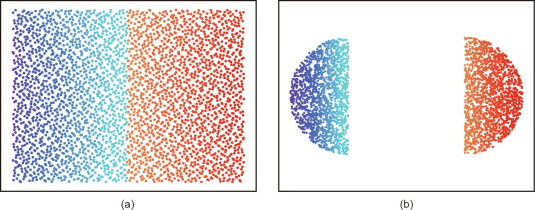
\includegraphics[width=0.6\linewidth]{9.jpg}
	\caption{不连续的OT映射,由基于Theorem\ref{theorem:4.2}的一个GPU算法实现生成。(a)源域;(b)目标域。(a)图中间的线代表的是奇异点集合$\sum_1$。}
	\label{fig:9}
\end{figure}

\begin{figure}[h]
	\centering
	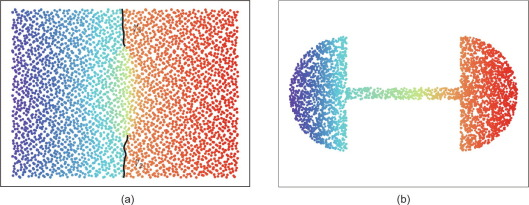
\includegraphics[width=0.6\linewidth]{10.jpg}
	\caption{不连续的OT映射,由基于Theorem \ref{theorem:4.2} 的一个GPU算法实现生成。(a)源域;(b)目标域。(a)图中的$\gamma_1$和$\gamma_2$是两个奇异点集合。}
	\label{fig:10}
\end{figure}

图\ref{fig:11}为$\mathbb{R}^3$中两个概率测度值之间的OT图。源测度$\mu$和目标测度$\nu$都是均匀分布;$\Omega$的支持是单位固体球,而$\Lambda
$的支持是固体斯坦福兔子。基于定理$\ref{theorem:4.2}$,我们计算了布雷尼尔势$u:\Omega \to \mathbb{R}$。为了可视化映射,我们插值概率测量如下:
\begin{equation*}
	\rho _t := \left [ (1-t)id+t\bigtriangledown \mu \right ]_{\#} \mu , 0 \le t \le 1 
\end{equation*}

图\ref{fig:11}为插值测量值$\rho_t$的支持度。表面上的折叠是奇点集,其中OT映射是不连续的。
\begin{figure}[h]
	\centering
	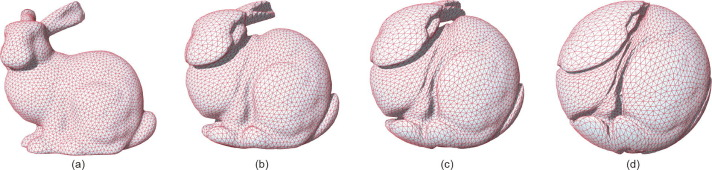
\includegraphics[width=0.6\linewidth]{11.jpg}
	\caption{从Stanford兔子到实心球的OT映射。边界曲面上的皱褶是奇异点集合。(a)~(d)显示了变化过程。}
	\label{fig:11}
\end{figure}

在一般情况下,由于真实数据分布、嵌入流形$\sum$和编码/解码映射的复杂性,目标测度量的支持度很少是凸的;因此,运输映射不能是全局连续的。

另一方面,一般的dnn,如ReLUdnn,只能近似于连续映射。由ReLUdnn表示的函数空间不包含所需的不连续传输映射。培训过程,或者,同样地,搜索过程将导致三种替代的情况:

(1) 训练过程不稳定,且不收敛。

(2) 搜索收敛于$\Lambda$的多个连通分量之一,并且映射收敛于所需的运输映射的一个连续分支。这意味着会遇到一个模式崩溃。

(3) 在培训过程中产生了一个交通地图,它成功地覆盖了所有的模式,但也覆盖了$\Lambda$以外的区域。在实际应用中,这将导致产生不现实的样本的现象,如图\ref{fig:12}的中间帧所示。
\begin{figure}[h]
	\centering
	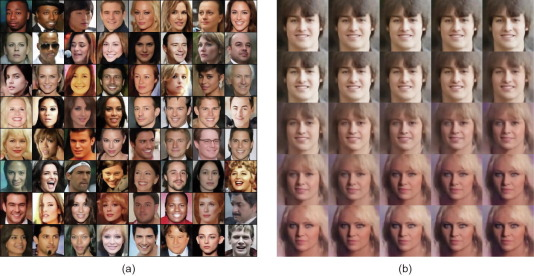
\includegraphics[width=0.6\linewidth]{12.jpg}
	\caption{AE-OT模型生成的人脸图像。(a)生成的实际人脸图像;(b)经过奇异点的路径。(b)图中心位置处的图像的传输映射是非连续的。}
	\label{fig:12}
\end{figure}


因此,在理论上,不可能直接使用DNN来近似OT映射。

\subsection{AE-OT模型}

如图\ref{fig:4}所示,我们分离了GANs的两个主要任务:流形学习和概率分布变换。第一个任务由AE执行,计算编码/解码映射$f_{\theta}, g_{\zeta}$;第二个任务是使用显式变分方法来计算潜在空间中的OT映射$T$。真实的数据分布v由编码映射$f_{\theta}$向前推进,诱导$(f_{\theta})_{\#} \nu$。在潜在空间中,$T$将均匀分布$\mu$映射到$(f_{\theta})_{\#} \nu$。

AE-OT模型有许多优点。在本质上,寻找OT映射是一个凸优化问题;保证了解的存在性和唯一性。采用拟牛顿方法,训练过程稳定且具有超线性收敛性。未知数的数量等于训练样本的数量,避免了过度参数化。并行OT映射算法可以使用GPU来实现。用蒙特卡罗方法可以通过采样密度来控制OT图的误差界。具有自适应能力的分层算法进一步提高了算法的效率。特别是,AE-OT模型可以消除模式崩溃。